\documentclass{beamer}

\mode<presentation> {
\usecolortheme{seagull}

\setbeamertemplate{footline}[page number]}
\usepackage{graphicx} 
\usepackage{booktabs} 
\usepackage{url}
\usepackage{hyperref}

\AtBeginSection[]{
  \begin{frame}
  \vfill
  \centering
    \usebeamerfont{title}\Huge{\insertsectionhead\par}
  \vfill
  \end{frame}
}

%-------------------------------------------------------------------------

\title[TLKDCC Machine descriptions and boot]{Machine descriptions and boot}
\author{Hans Holmberg}
\institute[LKTP]
{
Linux Kernel Teaching Project \\ 
\medskip
\textit{hans.holmberg@gmail.com}
}
\date{\today}
%------------------------------------------------------------------------
\begin{document}

\begin{frame}
\titlepage

\includegraphics{tux} 
\end{frame}

\begin{frame}
\frametitle{Overview}
\tableofcontents 
\end{frame}

%-----------------------------------------------------------------------
\section{Kernel boot process}

\begin{frame}
\frametitle{Bootstrapping}
\begin{itemize}
	\item The kernel cannot start itself on a system - a bootloader is needed to load the kernel from disk(or over the network,  a serial cable or usb, ..).
	\item The boot loader (that is usally bootstrapped as well) must initialize the system memory and load the kernel and provide the kernel with sufficent information to initialize the machine it is running on.
\end{itemize}
\end{frame}

\begin{frame}
\frametitle{Kernel boot process overview}
\includegraphics[width=\textwidth]{boot.pdf}
\end{frame}

\begin{frame}
\frametitle{Secure boot}
\begin{itemize}
	\item In order to keep malicious code from running in kernel space, the code and data must be verified to be from a trusted source.
	\item Verification is done using a chain of trust from the boot stages up to the kernel. Each component must cryptographically verify the next piece of code before executing it.
	\item Once the kernel is running, the kernel can verify all kernel modules it is loading, if you turn on the CONFIG\_MODULE\_SIG option \footnote{See module signing kernel documentation \url{https://www.kernel.org/doc/Documentation/module-signing.txt}\\}
\end{itemize}
\end{frame}

\begin{frame}
\frametitle{Kernel initialization}
\begin{enumerate}
	\item Early init - handle parameters passed on from the bootloader 
	\item Transition to protected mode (if x86)
	\item Decompression of kernel
	\item Page table and early interrupt and exception handling setup
	\item start\_kernel() \footnote{main.c \url{http://lxr.free-electrons.com/source/init/main.c} \\}
	\begin{enumerate}
		\item Perform arch−specific setup (memory layout analysis, copying boot command line again, etc.).
		\item Print Linux kernel "banner" containing the version  (early prints available now)
		\item Initialise traps, irqs, data required for scheduler.
		\item Parse boot command line options and initialise console. - (normal console prints available)
		\item Enable interrupts.
		\item Initialize memory allocation and print out the "Memory: ..." line.
		\item Perform arch−specific "check for bugs" and, whenever possible, activate workaround for processor/bus/etc bugs.
		\item Initialize scheduler, trigger start of init process
		\item Go to idle loop
	\end{enumerate}
\end{enumerate}
\end{frame}

\begin{frame}
\frametitle{Memory map (post-boot) example, 32bit, Virtual}
\begin{center}
\includegraphics[width=0.4\textwidth]{memorymap.pdf}
\end{center}
\end{frame}
%-----------------------------------------------------------------------
\section{Machine descriptions}

\begin{frame}
\frametitle{Machine descriptions definition}
Describing system hardware in a platform-independent manner
\begin{itemize}
	\item One kernel binary, many boards/platforms
	\item Non-auto-detectable stuff needs to be specified somehow
	\item Devices on non-enumerable buses
	\item Device properties
	\item Memory mapped registers
	\item GPIOs
	\item Regulators
	\item ..other board/soc/.. specifics
\end{itemize}
\end{frame}

\begin{frame}
\frametitle{Illustration}
\begin{center}
\includegraphics[width=0.8\textwidth]{descriptiontree.pdf}
\end{center}
\end{frame}

\begin{frame}
\frametitle{Devicetree vs ACPI}
\begin{itemize}
	\item Device tree
	\begin{itemize}	
		\tiny
		\item Keep it simple
		\item Mandatory for all new ARM SOCs 
		\item Machine description only (Flattened Device Tree)
		\item Tree structure written in DTS (Device Tree Source) format
		\item Compiler available in kernel tree
		\item Mainly embedded
		\item DTB Normally stored on main storage (eMMC / ..)
	\end{itemize}
	\item ACPI - Advanced Configuration and Power Interface
	\begin{itemize}
		\tiny
		\item Mainly x86/desktops/servers (but recently also in embedded stuff) 
		\item Feature rich 
		\item Aims to abstract the hardware from the OS
		\item Predominately x86 ...but support for ARM V8 added in the ACPI 5.1 spec
		\item Machine description (DSDT) + runtime services
		\item Tree structure written in ASL  (ACPI Source Language) format
		\item Separate(open source) compiler available
		\item Normally stored in firmware SPI NOR
	\end{itemize}
\end{itemize}
\end{frame}

\begin{frame}
\frametitle{Development flow}
\begin{itemize}
	\item Devicetree
	\begin{itemize}
		\item Update board .dts
		\item Build kernel, or just the dts
		\item Provision and reboot
		\item Commit result  
	\end{itemize}
	\item ACPI
	\begin{itemize}
		\item Grab the DSDT table cat /sys/firmware/acpi/tables/DSDT > dsdt.dat
		\item Decompile  iasl -d dsdt.dat 
		\item Enable  DSDT override (DSDT .hex included in kernel)
		\item Menuconfig: Device Drivers > Generic Driver Options > Include Custom DSDT
		\item Update dsdt.dsl (+kernel)
		\item Compile DSDT
		\item iasl -ic dsdt.dsl
		\item Build kernel, provision and reboot
		\item Update firmware 
	\end{itemize}
\end{itemize}
\end{frame}

\begin{frame}
\frametitle{Machine description examples}
\begin{itemize}
	\item Raspberry Pi 2B - arch/arm/boot/dts/bcm2709-rpi-2-b.dts
	\item Laptop - laptop\_dsdt.dsl
\end{itemize}
\end{frame}

%-----------------------------------------------------------------------
\section{Drivers}

\begin{frame}
\frametitle{What is a driver?}
A device driver:
\begin{itemize}
	\item Enables the operating system to interact with a piece of hardware.
	\item Aims to abstract the hardware specific properties away
	\item Provide access to it via an interface shared with other devices to a common kernel framework(i.e. input, iio, ..) 
\end{itemize}
\end{frame}


\begin{frame}
\frametitle{What is a driver?}
\begin{center}
\includegraphics[width=0.65\textwidth]{driverstack.pdf}
\end{center}
\end{frame}

\begin{frame}
\frametitle{Driver vs Device}
It is important to distinguish between drivers and devices:
\begin{itemize}
	\item Object oriented view: A driver is the class, a device is an object.
	\item Drivers provide code handling a class of hardware, device objects contain the specific state for a single piece of hardware.
	\item Drivers work as adapters between the hardware and the kernel framework the devices are attached to.
\end{itemize}
\end{frame}

\begin{frame}
\frametitle{Driver vs Device}
\begin{center}
\includegraphics[width=0.65\textwidth]{driver.pdf}
\end{center}
\end{frame}

\begin{frame}
\frametitle{Device types}
\begin{itemize}
	\item Block devices - access to raw storage
	\item Network devices - network interfaces
	\item Character devices - all others
\end{itemize}

%Major and minor number, used when creating files.
%Documentation/devices.txt
%All devices stored in /dev

\end{frame}

\begin{frame}
\frametitle{Drivers, devices and buses}
Drivers and devices are attached to a bus to communicate with the hardware.
\begin{itemize}
	\item Completely enumarable buses: PCI, USB, ..
	\item Semi-enumerable buses: I2C, SPI, ..
	\item Non-enumerable bus: platform devices
\end{itemize}
\end{frame}


\begin{frame}
\frametitle{Driver life cycle}
\begin{itemize}
	\item Init - global initialization
	\item Probe - create device
	\item Open / Close cycles
	\item Power management cycles
	\item Remove - global deinitalization
\end{itemize}
\end{frame}

\begin{frame}
\frametitle{Built in vs loadable modules}
\begin{itemize}
\item Code that does not need to be executed before a filesystem is available to the kernel can be compiled as a kernel module. \\
\item Kernel modules saves a lot of memory!
\item Modules can be loaded automatically, if the module provides a device table that can be matched with i.e usb device ids. \\
\end{itemize}
\end{frame}

\begin{frame}
\frametitle{Useful tools}
\begin{itemize}
	\item List loaded modules: lsmod
	\item Load module: insmod(single module), modprobe(resolves dependencies)
	\item Display module information: modinfo
	\item Generate module dependencies: depmod
	\item Driver module example: pl2303 serial converter\\
\end{itemize}
See the kernel documentation project for more (great) documentation on kernel modules \footnote{Linux Loadable Kernel Module HOWTO \url{http://www.tldp.org/HOWTO/html\_single/Module-HOWTO/}\\}.
\end{frame}

\begin{frame}
\frametitle{ACPI Driver example}
ACPI Battery driver
\begin{itemize}
	\item ID: PNP0C0D
	\item Source: drivers/acpi/button.c
\end{itemize}
\end{frame}

\begin{frame}
\frametitle{Devicetree example}
GPIO Regulator driver
\begin{itemize}
	\item ID: gpio-regulator
	\item Source: drivers/regulator/gpio-regulator.c
\end{itemize}
\end{frame}

%-----------------------------------------------------------------------

\begin{frame}
\Huge{\centerline{Thanks!}}
\end{frame}

\end{document} 
